% Created 2026-09-07 Mon 10:18
% Intended LaTeX compiler: pdflatex
\documentclass[presentation]{beamer}
\usepackage[utf8]{inputenc}
\usepackage[T1]{fontenc}
\usepackage{graphicx}
\usepackage{longtable}
\usepackage{wrapfig}
\usepackage{rotating}
\usepackage[normalem]{ulem}
\usepackage{amsmath}
\usepackage{amssymb}
\usepackage{capt-of}
\usepackage{hyperref}
\usetheme{default}
\author{Rick Wysocki}
\date{}
\title{Week 3 / Tuesday}
\hypersetup{
 pdfauthor={Rick Wysocki},
 pdftitle={Week 3 / Tuesday},
 pdfkeywords={},
 pdfsubject={},
 pdfcreator={Emacs 30.2 (Org mode 9.7.11)}, 
 pdflang={English}}
\begin{document}

\maketitle
\begin{frame}[label={sec:orgf981f55}]{Confucius}
Dates: 551-479
\end{frame}
\begin{frame}[label={sec:orgbcef24b}]{Confucius's Representations}
\begin{itemize}
\item Teacher
\item Political advisor
\item Editor
\item Philosopher
\end{itemize}
\end{frame}
\begin{frame}[label={sec:orgbff667c}]{Key Ideas}
\begin{itemize}
\item \emph{Ru} (trans. ritual)
\item Ethics
\item Politics
\end{itemize}

\begin{figure}[htbp]
\centering
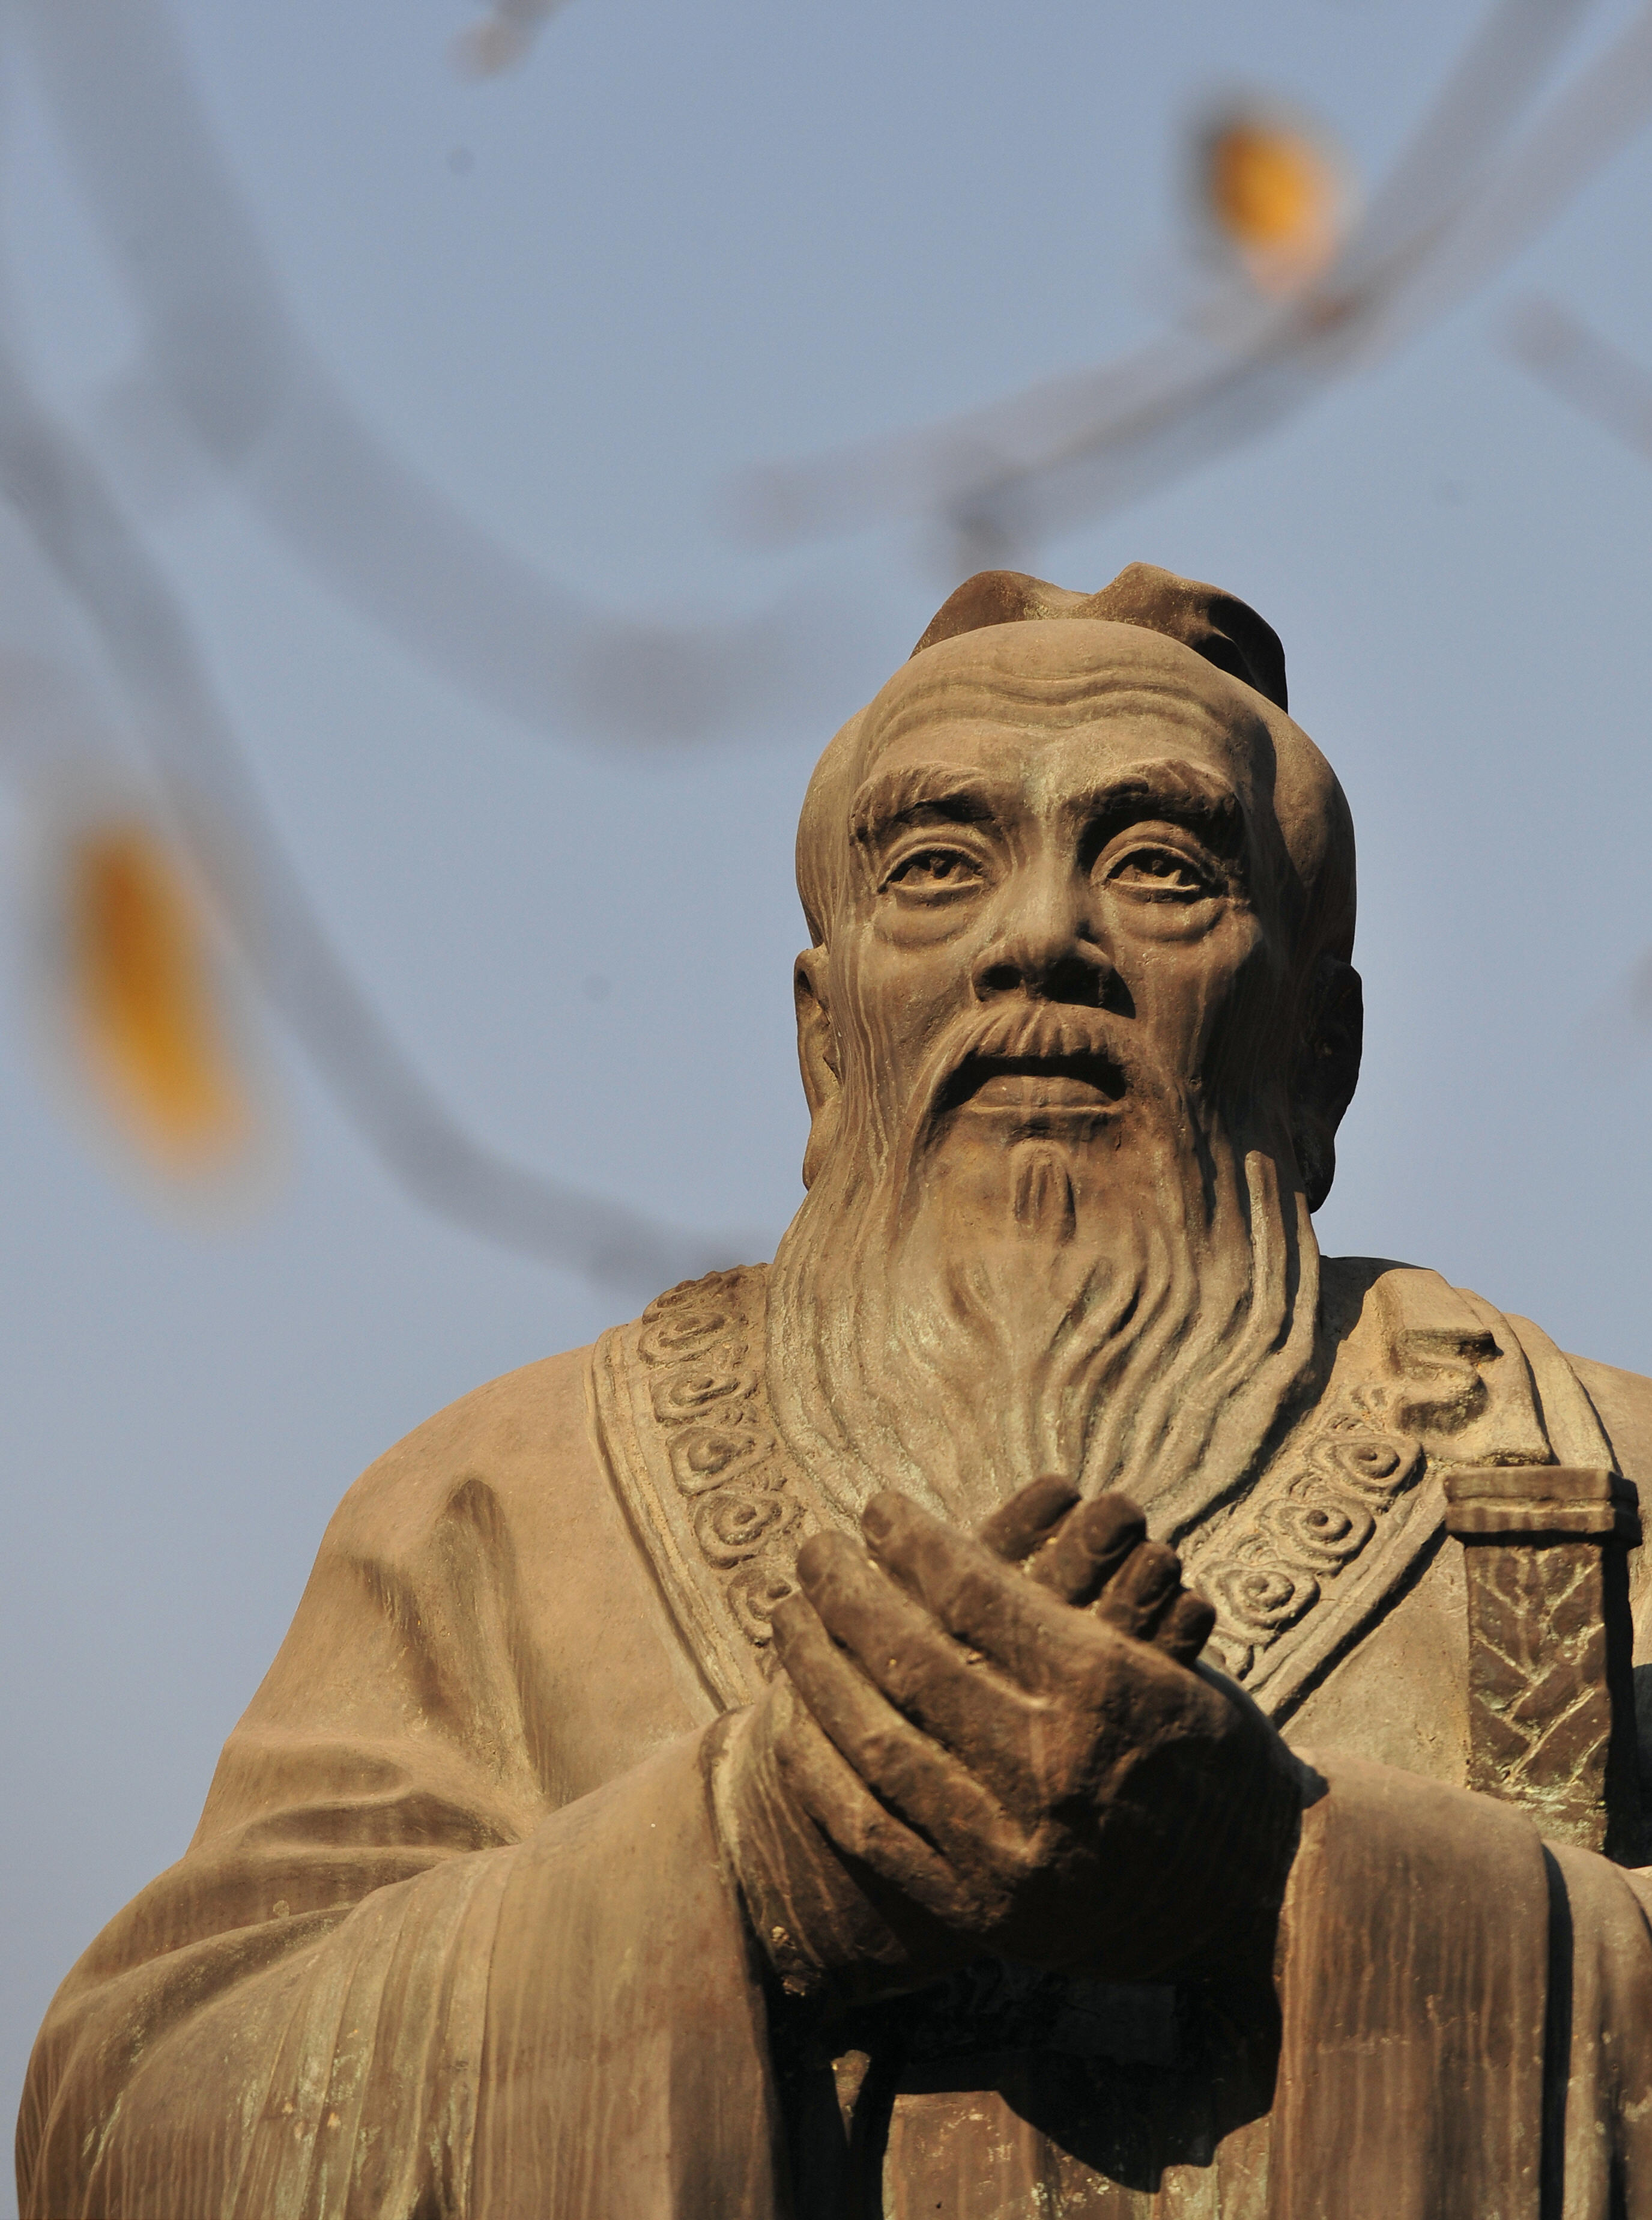
\includegraphics[trim=1cm 15cm 1cm 10cm, clip, width=0.7\textwidth,width=.9\linewidth]{./images/confucius-statue.jpg}
\caption{One representation of Confucius}
\end{figure}
\end{frame}
\begin{frame}[label={sec:org4d381e9}]{Social Context}
\begin{itemize}
\item Differing factions across China
\item Loss of public trust
\end{itemize}
\end{frame}
\begin{frame}[label={sec:orgd18f801}]{Location}
\begin{figure}[htbp]
\centering
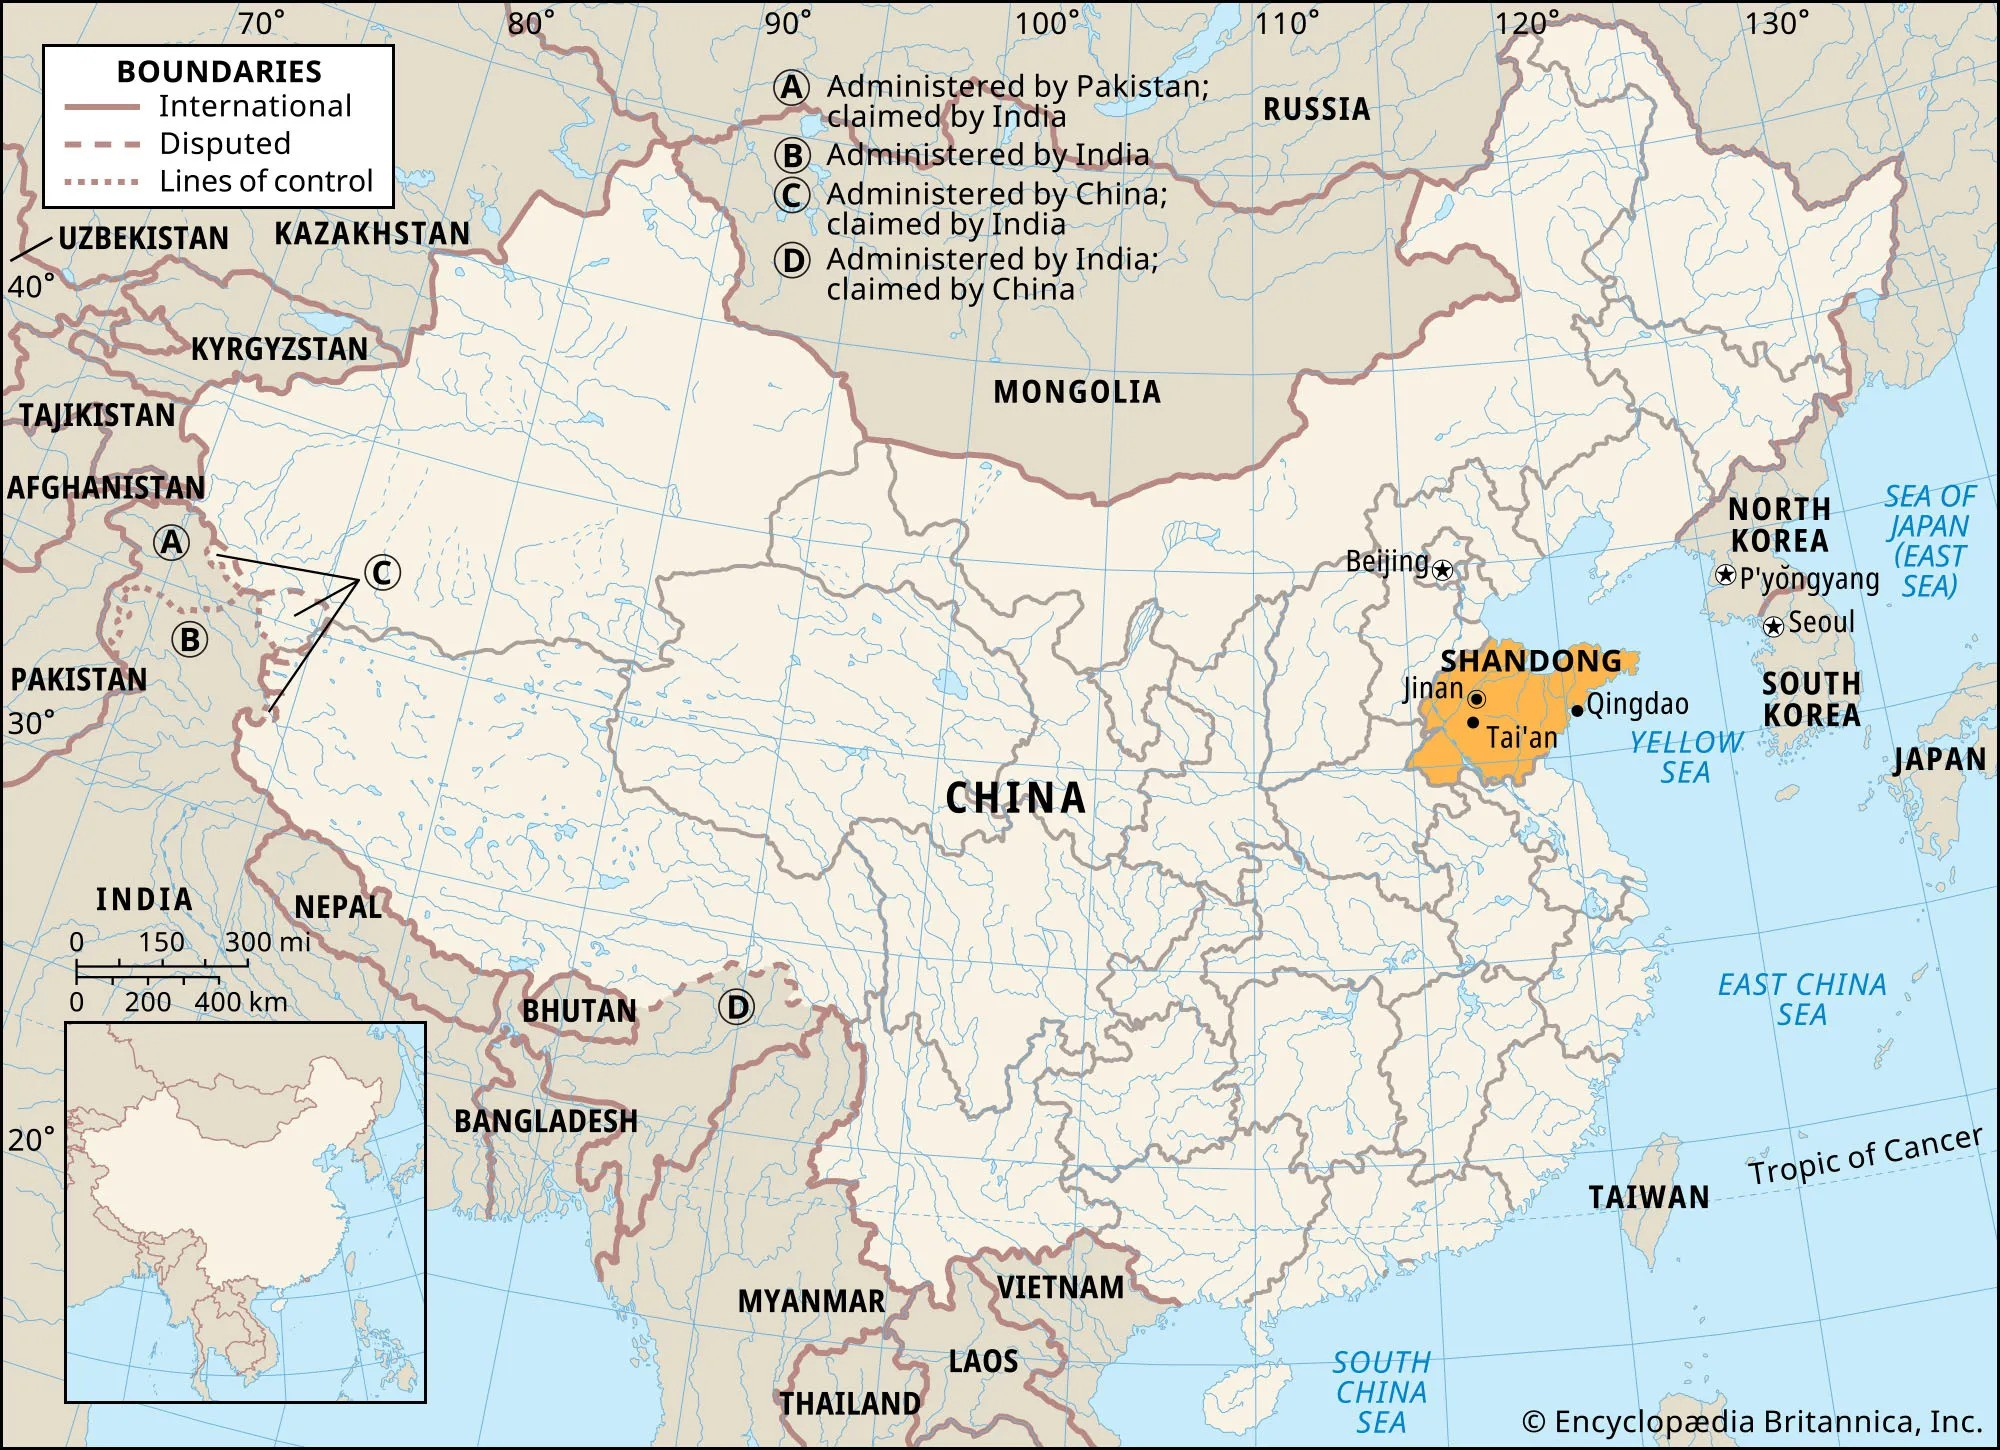
\includegraphics[width=.9\linewidth]{./images/shandong-map.jpeg}
\caption{Shandong's location in China.}
\end{figure}
\end{frame}
\begin{frame}[label={sec:orgfdfd0cf}]{Confucius's Project}
\begin{itemize}
\item Reintroduce social harmony
\item Appeal to culture/ritual
\item Train public officials to become better people to persuade others to do the same.
\end{itemize}
\end{frame}
\begin{frame}[label={sec:orgb75649a}]{Confucius's Project}
"Guide them by edicts, keep them in line with punishments, and the common people will stay out of trouble but will have no sense of shame. Guide them by virtue, keep them in line with the rites, and they will, besides having a sense of shame, reform themselves." (Chapter 2, Verse 3)
\end{frame}
\begin{frame}[label={sec:org8aa585a}]{Confucian View of Human Nature}
\begin{itemize}
\item Humans are fundamentally good
\item Cultural rituals (\emph{ru}) are a means of persuasion that develop and emphasize that goodness.
\end{itemize}
\end{frame}
\begin{frame}[label={sec:org012d4cc}]{\emph{Ru} / Ritual}
"Ritual is a unique, time-honored form of cultural communication. Human beings use particular ritual configurations to elevate or symbolically fix and recreate those beliefs that are important to them." (Xiaoye You, “The Way, Multimodality of Ritual Symbols, and Social Change: Reading Confucius’s Analects as a Rhetoric”)
\end{frame}
\begin{frame}[label={sec:org576575a}]{An Example}
"For example, according to the rite of wedding, the special occasion kicks off in a highly symbolic manner, When the representative of the bride's family appears afar, the usher goes inside to inform the host. Then the host dresses up and welcomes the guest outside the house. He prostrates himself in front of the guest, who does not need to do so but simply bows to the host. At the entrance to the family shrine, the guest bows three times. Upon the stairs, the host invites the guest three times to take steps first. The host lets the guest go up to the western end of the house, so the guest takes the stairs on the west side." (trans. by You)
\end{frame}
\begin{frame}[label={sec:org2317476}]{Heaven/The Way}
\begin{itemize}
\item \alert{Heaven:} (primarily) non-theistic; associated with the Good/transcendent morality
\item \alert{The Way"} carrying out human actions in a way that puts you in harmony with "Heaven"
\end{itemize}
\end{frame}
\begin{frame}[label={sec:org6cea5de}]{Five Virtues}
\begin{itemize}
\item Benevolence
\item Righteousness
\item Ritual Propriety
\item Wisdom
\item Trustworthiness
\end{itemize}
\end{frame}
\begin{frame}[label={sec:orgf1fafc0}]{Benevolence}
Examples:
\begin{itemize}
\item Treating the homeless as guests in one’s home
\item Rejecting clever speech
\item Being hesitant to speak
\item Unselfishness
\end{itemize}
\end{frame}
\begin{frame}[label={sec:orgc8a159e}]{Righteousness}
Fitting one’s role in society in the appropriate way.

Contexts:
\begin{itemize}
\item In personal life: act in a way that one should act towards one's family.
\item In public/official life: act out of authentic respect for those of different social statuses, always resisting temptations for personal gain.
\end{itemize}
\end{frame}
\begin{frame}[label={sec:org5c38e3c}]{Ritual Propriety}
Approaching the rituals of culture with the correct and respectful mindset.
\end{frame}
\begin{frame}[label={sec:org53a9ebc}]{Wisdom}
"In the Analects, wisdom allows the gentleman to discern crooked and straight behavior in others. . . . In certain dialogues, wisdom also connotes a moral discernment that allows the gentleman to be confident of the appropriateness of good actions." (Stanford Encyclopedia of Philosophy)
\end{frame}
\begin{frame}[label={sec:orgc6f5251}]{Trustworthiness}
"To be trustworthy in word is close to being moral in that it enables one's words to be repeated." (Chapter 1, Verse 13)
\end{frame}
\begin{frame}[label={sec:orge4a8dce}]{Confucian Rhetoric}
\begin{itemize}
\item The truthful representation of reality
\item A discounting of argument in favor of social bonds
\end{itemize}
\end{frame}
\begin{frame}[label={sec:orgcad9a74}]{Confucian Rhetoric}
\begin{itemize}
\item " I can speak to Hui all day without his disagreeing with me in any way. Thus he would seem to be stupid. However, when I take a closer look at what he does in private after he has withdrawn from my presence, I discover that it does, in fact, throw light on what I said. Hui is not stupid after all." (Chapter 2, Verse 9)
\item "In antiquity men were loath to speak. This was because they counted it shameful if their person failed to keep up with their words." (Chapter 4, Verse 22)
\end{itemize}
\end{frame}
\begin{frame}[label={sec:orgb8005b9}]{Confucian Persuasion}
"The Goodness possessed by a gentleman was analogized as the power of breeze, which bends the glass but does not break it." (Xiaoye You)
\end{frame}
\begin{frame}[label={sec:org70d09c8}]{Gender in Confucian Thinking}
\end{frame}
\end{document}
